\section{Multi view optimization}


In the previous sections, we have shown how SQL queries can be 
translated into a query DAG (i.e. maintenance plan). Now, we are ready 
to tackle the multi view problem. Imagine an application or warehousing
system that encounters a large number and variety of different SQL 
queries. Using the naive approach, as described before, would mean
that every query would translate to its own set of materialized views
without sharing any intermediate results. To improve performance and
reduce the storage overhead a lot, we need a query optimizer; the 
optimizer has to find a global maintenance plan which is optimal 
with regard to total throughput and storage usage (or some other cost
parameters). 




\subsection{Cost model}


The cost model has to trade-off the different aspects of incremental
view maintenance. On the one side, there is the throughput of
maintenance operations (which determines the freshness of the data in
the view). A client operation triggers multiple updates along the 
maintenance plan. Depending on the amount and type of view expressions 
a specific number of view updates is generated. On the other side, there 
is the storage cost of hosting the intermediate and resulting view tables. 
The more intermediate tables are hosted, the more storage space is 
occupied. Therefore, we aim at reducing the number of intermediate views 
as much as possible. Whenever, we can possibly execute multiple operations 
on the same table, we combine them.

Both types of cost are expressed in out cost model: the processing or 
maintenance cost and the storage cost. The maintenance cost can be 
described by the number of operations (i.e. get, put and delete) per 
time interval $t$ that the VMS needs to execute to keep the view records 
up-to-date. The rate of operations depends on the view expressions, 
thus, we compute it by iterating over the expression nodes in the 
maintenance plan. First, we define the cost over a single  
vertex $v \in V$ as $c(v)$. The equation is given as follows: 



\begin{equation} 
\begin{aligned} 	   
   c(v)=&\underbrace{(i(v)+u(v)+d(v))*w_g}_\text{get} \\ 
   &+\underbrace{(i(v)+u(v))*w_p}_\text{put} +\underbrace{(d(v)+u(v))*w_d}_\text{delete}
\end{aligned}
\end{equation}

The equation computes the cost of all get, put and delete operations 
that are required to update the subsequent view table. The get part sums 
all get operations and multiplies them with $w_g$, which is a weight 
factor. For all incoming operations, a get-operation has to be performed 
on the view table. This way, the VM retrieves the old view record such 
that it can add the delta on top of it. In some cases, get operations 
are not needed at all (e.g. if a selection view follows a delta view). 
Then, the get-part of the equation can be set to zero. Since KV-stores 
are write optimized data bases -- and, thus, execute writes faster than 
reads -- we also use weight factors $w_p$ and $w_d$ for put and delete 
operations. Update operations can always be substituted by an insert 
plus a delete operation. Thus they are included in the put part, as well 
as the delete part of the equation. 

The functions $i(v)$, $u(v)$ and $d(v)$ deliver the rate of insert, 
update and delete operations that the vertex receives from all its 
direct predecessors. Since the predecessors are table or expression 
nodes, whose input, again, may depend on preceding nodes, we define the 
input rate $i(v)$ recursively. 



\begin{equation} 
\begin{aligned} 	   
	i(v)=& \sum_{v \in pred(v_x)}&i(v)\;\;\; if \; pred(v) \neq \emptyset \\
	i(v)=& &\lambda_i(v)\;\;\; if \: pred(v) = \emptyset
\end{aligned}
\end{equation}


If the set of predecessors is not empty, the sum of input rates over them
is computed. If the set of predecessors is empty, the node must be a base 
table. Then, function $\lambda_i(v)$ represents the rate of operations that 
are applied to the base table. The input rate at the base tables
is either provided to VMS as a meta parameter or has to be determined in
a test run, before actual view maintenance is performed. The equations
to compute update $u(v)$ and delete $d(v)$ rates can be formulated accordingly.

Having the processing cost evaluated we still need to compute the estimated
maximum storage cost. The following general formula works for all view table
nodes:

\begin{equation} 
\begin{aligned} 	   
   c(v)=r(v)*f(v)
\end{aligned}
\end{equation}

%\prod_{v_x \in pred(v_t)} f(v_x)

The input is a table vertex $v \in V$. The function $r(v)$ evaluates
the number of records in the table. Again, the number of records in 
tables can be defined recursively over the maintenance plan as:

\begin{equation} 
\begin{aligned} 	   
	r(v)=& \sum_{v \in pred(v)}&r(v)\;\;\; if \; pred(v) \neq \emptyset \\
	r(v)=& &\mu(v)\;\;\; if \: pred(v) = \emptyset
\end{aligned}
\end{equation}


\begin{figure*} \centering 
	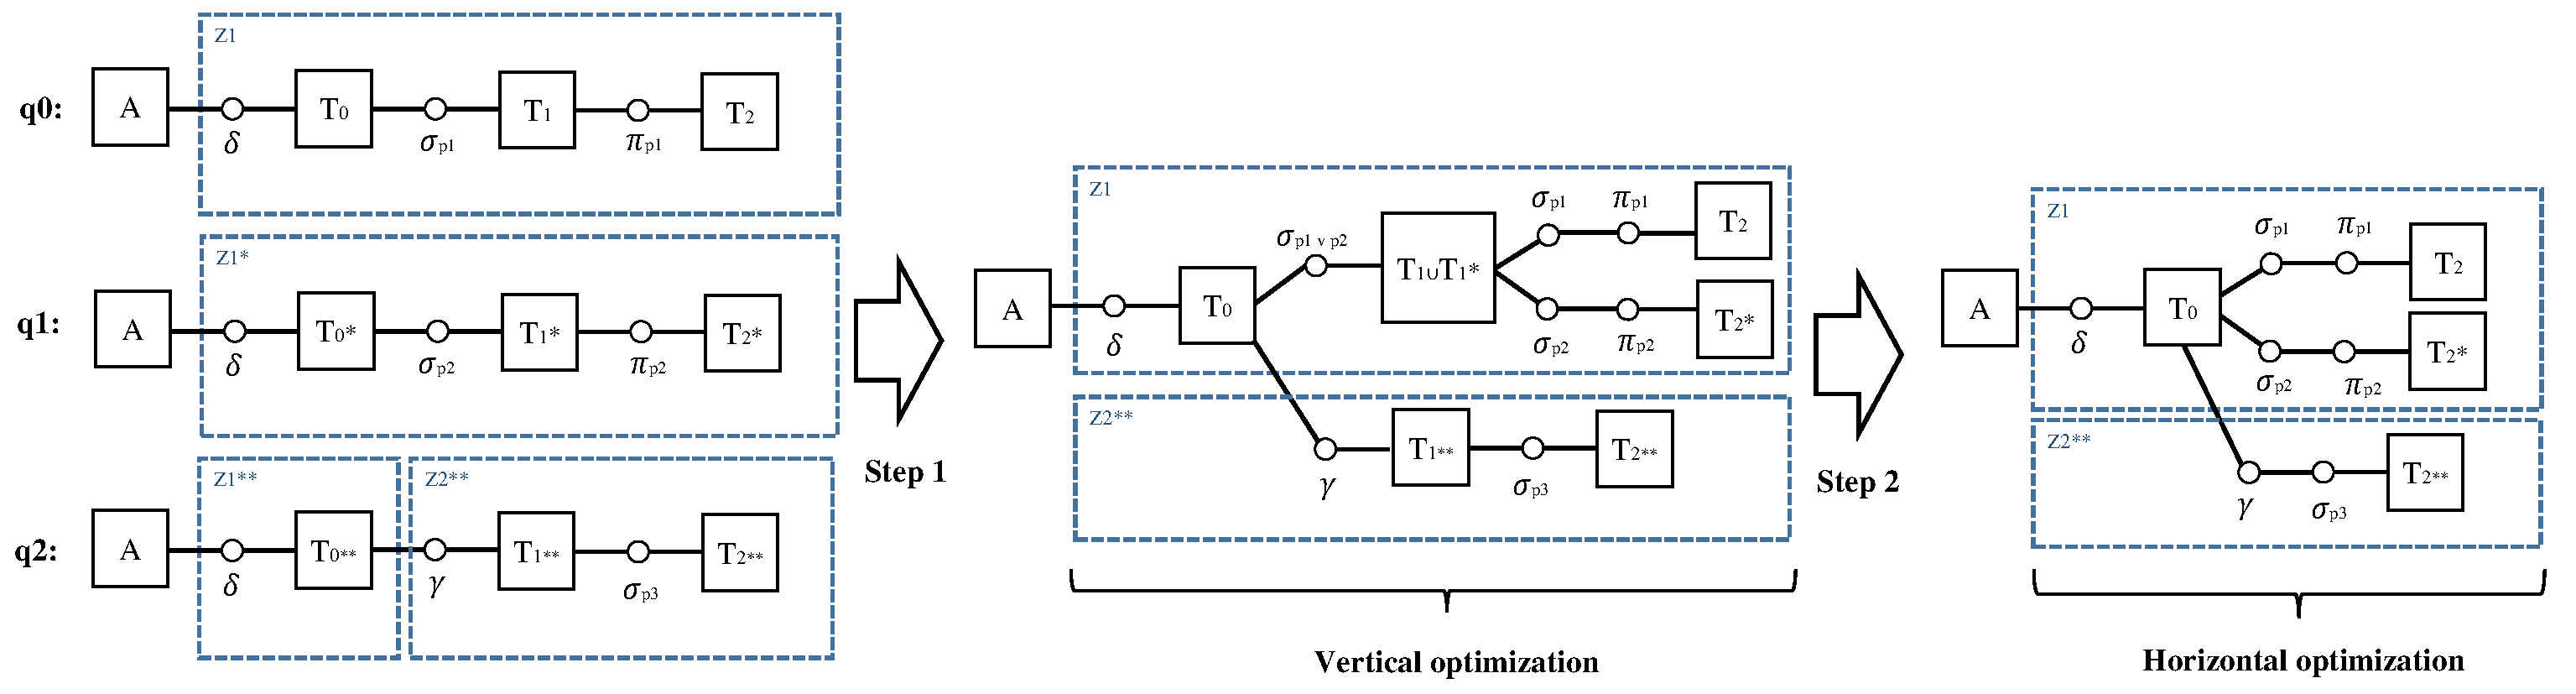
\includegraphics[width=\linewidth]{figures/VerticalOptimization} 
	\caption{Multi-query optimization} \label{fig:vertical_optimization} 
\end{figure*} 

The number of records is defined as the sum of records from the nodes 
predecessors, unless it is a base table. Then,
the function $\mu(v)$ delivers the average number of records. Again, this
number is either given or has to be estimated.
Based on the number of records in the base table, the number of records in 
the view tables can be computed. The number has to be multiplied with a 
factor $f(v)$. The factor expresses that, depending on the view expression,
a the number of view records can be larger or smaller than in the base table.
A selection expression e.g., reduces the amount of records in the view table
depending on the selection predicate. A join can possibly increase the
number of records, e.g. when the cross product of two tables is built. Thus
the function $f(v)$ is denoted as the product of factors from all view 
expressions that are direct predecessors of the node $predX(v)$. The factor, 
represented by function $\psi(v_x)$ has to be given or needs to be evaluated
in a test run.


\begin{equation} 
\begin{aligned} 	   
	f(v)=& \prod_{v_x \in predX(v)}&\psi(v_x)\\
\end{aligned}
\end{equation}


Now, we have defined the cost of table, as well as expression
vertices, we are ready to compute the total cost of the maintenance plan. It is
done as follows:

\begin{equation} 
\begin{aligned} 	   
   c(p)=\sum_{v_x \in V_x(p)} c(v_x)*w_x + \sum_{v_t \in V_T(p)} c(v_t)*w_t
\end{aligned}
\end{equation}

In order to compute the cost of the graph, we need to evaluate the sum 
of the cost of all nodes. Because the cost is based on throughput of client
operations, and nodes are depending on each other (i.e. one node my reduce
the throughput of the next one), the maintenance plan needs to be traversed 
starting at the base tables. Thus, we apply a graph traversing algorithm (e.g. 
Kahn's algorithm) to determine a topology of the graph (i.e. an ordered
according to the placement in the graph). This can be done with linear 
complexity. Then, we follow the topology and compute the throughputs and
storage cost of all nodes iteratively. Finally, we obtain the overall sum
of the maintenance plan $c(p)$.



\subsection{Vertical optimization}

The optimization algorithm operates on a set of query DAGs. In section
before, we merged table nodes within a zone of a single query pattern;
we called it horizontal optimization. Now, we also consider merging table 
nodes of different maintenance plans from different queries; we call it 
vertical optimization.

Figure~\ref{fig:vertical_optimization} depicts the process of vertical 
optimization (and subsequent horizontal optimization). On the left side 
of the figure, three separate maintenance plans of three different 
queries are shown (i.e. $q_0$, $q_1$ and $q_2$). These plans are 
directly derived from the corresponding SQL statements: 



\begin{enumerate}
	\item $q_0$ $\leftarrow$ Select $c_1$ from $A$ where $p_1$ 
	\item $q_1$ $\leftarrow$ Select $c_2$ from $A$ where $p_2$ 
	\item $q_2$ $\leftarrow$ Select Sum($c_2$) from $A$ group by $c_1$ having $p_3$
\end{enumerate}


In Step~1, multiple vertical merges are executed on the plans, which
leads to the graph in the center of the figure. The algorithm starts
at the base tables (i.e. $A$) and merges in a zipper-like fashion 
along the view chain. As a first sub-step all base tables (i.e. all $As$) 
can be merged together. The nodes are identified by name; we take the
first node of $q_1$ as base table node and remove the base table nodes
of $q_1$ and $q_2$. Further, we redirect the outgoing edges of both 
maintenance plans.
As a second sub-step, all delta views (i.e. $T_0$,
$T_0*$ and $T_0**$) are merged together. Since the delta expression 
for all three views is the same, we proceed exactly as before. We
 


\noindent
\textbf{Merging equal expressions}





For the merging of two (or more) table nodes of two (or more) query DAGs,
some preconditions have to be fulfilled: (1) the table node is either
computed from the same expression (e.g. $\sigma_{c_1 = 10}(A)$) or it is
computed from a similar expression of the same operator (e.g $\sigma_{c_1 
< 10}(A)$ and $\sigma_{c_1 > 5}(A)$); thereby, the two expressions need
at least a set of intersection records. Otherwise, it makes no sense to
merge them. (2) the derivation of both tables has to be the same (aside 
from the merged expression). For example, if we merge two aggregation
expressions, then the preceding expressions (e.g. delta, selection) have 
to match exactly.   



Merging equal view tables is always advantageous. Instead of two tables
we just use one, thus, we save storage and processing capacity. 

\noindent
\textbf{Merging similar expressions}


\subsection{Problem definition}

As a first step towards the solution, we formalize the 
problem as follows: 

Given a set of $n$ queries $q_n$ and the corresponding
set of maintenance plans $p_n \in P$: what is the global maintenance
plan $p_g$ that executes all plans $p_n$ and is optimal with 
regard to overall cost.  




\subsection{Optimization algorithm}



Now that we have defined the types of possible merge operations (i.e. 
horizontally and vertically) and also constrained the cost model, we
discuss the optimization algorithm. The first version of our algorithm 
will work in three iterative steps: (1) the algorithm optimizes 
vertically; it finds all equal expressions and table nodes and merges 
them, without cost evaluation. (2) the algorithm optimizes vertically;
it finds all similar expressions and table nodes and merges them based
on cost estimation. (3) the algorithm optimizes horizontally; it uses
the resulting query DAG from the steps before and condenses it further.


\begin{algorithm}
\caption{Multi view optimization}
\label{alg:assignvm}
\begin{algorithmic}[5]
\Procedure{$optimize$}{$P_{Q}$}\Comment{$P_Q$ is a set of plans}
\State $V_G \leftarrow findEqualGroups(P_{Q})$\Comment{Step 1}
\ForAll{$v_g \in V_G$}
\State $P_{Q} \leftarrow verticalMerge(v_g)$	
\EndFor
\State $V_G \leftarrow findSimilarGroups()$\Comment{Step 2}	
\ForAll{$v_g \in V_G$}
\State $benefitial \leftarrow c(verticalMerge(v_g)) < c(v_g) $
\If{$benefitial$}	
\State $P_{Q} \leftarrow verticalMerge(v_g)$
\EndIf	
\EndFor
\State $V_G \leftarrow findZones()$
\ForAll{$v_g \in V_G$}\Comment{Step 3}	
\State $P_{Q} \leftarrow horizontalMerge(v_g)$	
\EndFor
\EndProcedure
\end{algorithmic}
\end{algorithm}


%We define a group as $G=\{{P_Q'}_1..{P_Q'}_n\}$, where $P_Q' \subseteq P_Q$.
%
%\begin{algorithm}
%\caption{Multi view optimization}
%\label{alg:assignvm}
%\begin{algorithmic}[5]
%\Procedure{$optimize$}{$P_{Q}$}\Comment{$P_Q$ is a set of plans}
%
%\State $list_G \leftarrow findCandidateGroups(P_{Q})$\Comment{partitions}
%\ForAll{$g \in list_G$}
%\ForAll{$P_Q' \in g$}
%\If {$mergePossible(P_Q')$}	
%\State $P_Q' \leftarrow verticalMerge(P_Q')$
%\State $P_Q' \leftarrow horizontalMerge(P_Q')$
%\Else
%\State $removeGroup(list_G, g)$	
%\EndIf
%\EndFor
%\If {$c(g) < c(best_g)$}
%\State $best_g \leftarrow g$
%\EndIf
%\EndFor
%
%\Return {$best_g$}
%\ForAll{$v_g \in V_G$}\Comment{Step 3}	
%\State $P_{Q} \leftarrow horizontalMerge(v_g)$	
%\EndFor
%
%
%
%\State $V_G \leftarrow findSimilarGroups()$\Comment{Step 2}	
%\ForAll{$v_g \in V_G$}
%\State $benefitial \leftarrow c(verticalMerge(v_g)) < c(v_g) $
%\If{$benefitial$}	
%\State $P_{Q} \leftarrow verticalMerge(v_g)$
%\EndIf	
%\EndFor
%\State $V_G \leftarrow findZones()$
%
%\EndProcedure
%\end{algorithmic}
%\end{algorithm}


\subsection{Complexity}




